\documentclass[11pt,a4paper]{article}

% ---- Nature-style packages ----
\usepackage[margin=2.5cm]{geometry}
\usepackage{times}
\usepackage[numbers,sort&compress]{natbib}
\usepackage{graphicx}
\usepackage{tikz}
\usetikzlibrary{shapes.geometric, arrows.meta, positioning, calc, fit, backgrounds}
\usepackage{booktabs}
\usepackage{multirow}
\usepackage{hyperref}
\usepackage{xcolor}
\usepackage{enumitem}
\usepackage{caption}
\usepackage{subcaption}
\usepackage{amsmath,amssymb}
\usepackage{float}
\usepackage{fancyhdr}
\usepackage{mdframed}
\usepackage{titlesec}

% ---- Nature colors ----
\definecolor{natureblue}{RGB}{0,102,153}
\definecolor{naturegray}{RGB}{100,100,100}
\definecolor{natureboxbg}{RGB}{240,245,250}
\definecolor{natureboxborder}{RGB}{0,102,153}
\definecolor{expertsred}{RGB}{200,60,60}
\definecolor{expertsgreen}{RGB}{60,160,80}
\definecolor{expertsblue}{RGB}{60,100,180}
\definecolor{expertsgold}{RGB}{200,160,40}
\definecolor{gatepurple}{RGB}{120,60,160}

\hypersetup{
  colorlinks=true,
  linkcolor=natureblue,
  citecolor=natureblue,
  urlcolor=natureblue
}

% ---- Section formatting (Nature style) ----
\titleformat{\section}{\Large\bfseries\sffamily}{\thesection}{1em}{}
\titleformat{\subsection}{\large\bfseries\sffamily}{\thesubsection}{1em}{}
\titleformat{\subsubsection}{\normalsize\bfseries\sffamily}{\thesubsubsection}{1em}{}

% ---- Header/Footer ----
\pagestyle{fancy}
\fancyhf{}
\fancyhead[L]{\small\color{naturegray}\textsf{Nature Reviews | Bioengineering}}
\fancyhead[R]{\small\color{naturegray}\thepage}
\renewcommand{\headrulewidth}{0.4pt}
\renewcommand{\headrule}{\hbox to\headwidth{\color{natureblue}\leaders\hrule height \headrulewidth\hfill}}

% ---- Key Points box ----
\newenvironment{keypoints}{%
  \begin{mdframed}[
    backgroundcolor=natureboxbg,
    linecolor=natureboxborder,
    linewidth=1pt,
    roundcorner=5pt,
    innertopmargin=10pt,
    innerbottommargin=10pt,
    innerleftmargin=15pt,
    innerrightmargin=15pt
  ]
  \noindent\textbf{\textsf{Key Points}}\par\medskip
  \begin{itemize}[leftmargin=15pt, itemsep=3pt]
}{%
  \end{itemize}
  \end{mdframed}
}

% ---- Title ----
\title{
\vspace{-1cm}
\textsf{\textbf{\Large Mixture of Experts in Healthcare:\\[4pt] From Conditional Computation to Clinical Intelligence}}
\vspace{0.3cm}
}

\author{
\textsf{Review Article}
\vspace{0.2cm}
}

\date{}

\begin{document}
\maketitle
\thispagestyle{fancy}

% ---- Abstract ----
\begin{abstract}
\noindent
Mixture of Experts (MoE) architectures have emerged as a transformative paradigm in artificial intelligence, enabling the scaling of model capacity while maintaining computational efficiency through conditional activation of specialized sub-networks. Originally proposed three decades ago, MoE has experienced a renaissance driven by advances in deep learning and the demands of processing heterogeneous, multi-modal healthcare data. This Review examines the rapidly expanding application of MoE across the healthcare spectrum, encompassing medical imaging and computational pathology, clinical natural language processing and medical large language models, drug discovery and genomics, electronic health records analysis, and multi-modal clinical decision support. We discuss the architectural innovations that make MoE particularly suited to healthcare challenges, including its ability to handle data heterogeneity, capture disease subtypes, and integrate diverse data modalities. We further address critical challenges including interpretability, expert collapse, clinical validation, and regulatory considerations. Finally, we outline future directions at the intersection of MoE and precision medicine, including personalized expert routing, federated MoE training, and the integration of MoE into clinical foundation models.
\end{abstract}

\vspace{0.5cm}

% ---- Key Points Box ----
\begin{keypoints}
  \item MoE architectures enable conditional computation by activating only a subset of specialized expert sub-networks for each input, decoupling model capacity from inference cost.
  \item In healthcare, MoE naturally addresses data heterogeneity across imaging modalities, clinical specialties, and patient populations by routing inputs through domain-specialized experts.
  \item MoE has been successfully applied to medical imaging (pathology, radiology, segmentation), clinical NLP and medical LLMs (diagnosis support, hallucination reduction), drug discovery, EHR analysis, and multi-modal clinical decision support.
  \item Key challenges include interpretability of routing decisions, expert collapse in imbalanced medical datasets, regulatory validation of modular AI systems, and data privacy constraints.
  \item Future directions include personalized expert routing for precision medicine, federated MoE training across institutions, and integration into clinical foundation models.
\end{keypoints}

\vspace{0.5cm}


\section*{Introduction}
\addcontentsline{toc}{section}{Introduction}

The healthcare sector generates vast quantities of heterogeneous data, from high-resolution medical images and longitudinal electronic health records to genomic sequences and clinical narratives. While deep learning has achieved remarkable success across these domains, the conventional paradigm of training monolithic, dense models faces fundamental scalability constraints: increasing model capacity uniformly activates all parameters for every input, resulting in prohibitive computational costs that limit deployment in resource-constrained clinical environments \cite{kaplan2020scaling}. The Mixture of Experts (MoE) architecture offers an elegant solution to this dilemma by enabling \textit{conditional computation}, where only a subset of model parameters is activated for each input, thereby decoupling total model capacity from inference cost \cite{jacobs1991adaptive, shazeer2017outrageously}.

The core insight of MoE aligns naturally with the structure of medical data and clinical reasoning. Diseases manifest differently across patients, imaging modalities capture complementary anatomical information, and clinical decision-making inherently involves consulting domain-specific knowledge. An MoE framework mirrors this structure by routing each input to specialized expert sub-networks, each potentially capturing distinct patterns corresponding to disease subtypes, tissue morphologies, imaging artifacts, or patient demographics \cite{masoudnia2014mixture}. This conditional activation paradigm has proven especially valuable in healthcare, where data distributions are long-tailed, class imbalances are severe, and the cost of errors can be life-threatening.

Recent years have witnessed an explosive growth in MoE-based approaches for healthcare applications. In medical imaging, MoE architectures have been deployed to handle variable image quality, multi-site heterogeneity, and multi-task segmentation \cite{rahman2025personalized_moe, xie2024moe_pathology}. In clinical natural language processing, MoE layers have been integrated into large language models (LLMs) to specialize different experts for distinct medical sub-domains, improving diagnostic reasoning while reducing hallucination \cite{bechar2025biocancer_moe, chen2026cor_mole}. In drug discovery, MoE frameworks have enabled joint modeling of diverse molecular properties and multi-scale biological representations \cite{acharya2025mobius}. In electronic health record (EHR) analysis, MoE-based multi-task learning has simultaneously predicted multiple clinical outcomes by routing patient records through task-specific experts \cite{rajkomar2018ehr_deep}.

This Review provides a comprehensive examination of MoE architectures applied to healthcare. We begin by establishing the mathematical and architectural foundations of MoE, including gating mechanisms, expert specialization strategies, and load balancing. We then systematically survey applications across five major healthcare domains: medical imaging and computational pathology, clinical NLP and medical LLMs, drug discovery and genomics, EHR analysis, and multi-modal clinical decision support. We critically evaluate the unique challenges that arise when deploying MoE in clinical settings, including interpretability requirements, regulatory considerations, expert collapse, and data privacy constraints. We also outline future directions where MoE architectures may fundamentally reshape clinical AI, including personalized routing, federated expert training, and integration into healthcare foundation models.


\section*{Foundations of Mixture of Experts}
\addcontentsline{toc}{section}{Foundations of Mixture of Experts}

\subsection*{The original MoE formulation}

The Mixture of Experts architecture was introduced by \cite{jacobs1991adaptive} as a modular neural network comprising multiple expert networks and a gating network that learns to partition the input space. Given an input $\mathbf{x}$, the MoE output is computed as:

\begin{equation}
    y = \sum_{i=1}^{N} g_i(\mathbf{x}) \cdot E_i(\mathbf{x})
\end{equation}

\noindent where $N$ is the number of experts, $E_i(\mathbf{x})$ denotes the $i$-th expert network, and $g_i(\mathbf{x})$ represents the gating weight assigned by the gating network $G$, typically implemented as a softmax over linear projections:

\begin{equation}
    g_i(\mathbf{x}) = \frac{\exp(\mathbf{w}_i^\top \mathbf{x})}{\sum_{j=1}^{N} \exp(\mathbf{w}_j^\top \mathbf{x})}
\end{equation}

This formulation enables the model to learn a soft partitioning of the input space, where different experts specialize in different regions or data patterns. The key theoretical advantage is that each expert needs to model only a subset of the data distribution, reducing the complexity of the learning problem for individual components while the ensemble maintains global expressiveness \cite{yuksel2012twenty}.

\subsection*{Sparse MoE and conditional computation}

The modern revival of MoE was catalyzed by the seminal work of \cite{shazeer2017outrageously}, who introduced the sparsely-gated MoE layer that activates only the top-$k$ experts for each input token. This sparse routing mechanism fundamentally changed the scalability equation: a model with $N$ experts and top-$k$ routing ($k \ll N$) can increase total parameter count by $N$-fold while increasing per-token computation by only $k/N$. The top-$k$ gating function is defined as:

\begin{equation}
    y = \sum_{i \in \text{TopK}(G(\mathbf{x}), k)} g_i(\mathbf{x}) \cdot E_i(\mathbf{x})
\end{equation}

\noindent where $\text{TopK}(\cdot, k)$ selects the $k$ experts with the highest gating scores. This approach enabled the training of models with trillions of parameters, such as the Switch Transformer \cite{fedus2022switch}, while maintaining inference costs comparable to much smaller dense models.

\subsection*{Load balancing and expert utilization}

A critical challenge in MoE training is ensuring balanced utilization of all experts. Without explicit regularization, the gating network tends to converge to a state where a small number of experts receive the majority of inputs (``rich get richer'' dynamics), leading to expert collapse where most experts remain undertrained. To address this, auxiliary load-balancing losses have been proposed:

\begin{equation}
    \mathcal{L}_{\text{balance}} = N \cdot \sum_{i=1}^{N} f_i \cdot P_i
\end{equation}

\noindent where $f_i$ is the fraction of tokens dispatched to expert $i$ and $P_i$ is the average gating probability for expert $i$ \cite{fedus2022switch}. Recent innovations include expert-level dropout \cite{zoph2022st}, capacity factors that limit the maximum number of tokens per expert, and hash-based routing that guarantees uniform assignment \cite{roller2021hash}.

\subsection*{MoE in the transformer era}

The integration of MoE into transformer architectures \cite{vaswani2017attention} has been the primary driver of recent advances. In transformer-based MoE models, the feed-forward network (FFN) layers in selected transformer blocks are replaced with MoE layers, where each ``expert'' is itself an FFN. This design preserves the attention mechanism for contextual token mixing while introducing conditional computation in the position-wise transformation. Key architectural variants include:

\textbf{Switch Transformer} \cite{fedus2022switch}: simplifies MoE routing to top-1 (each token sent to a single expert), dramatically simplifying the design while maintaining performance.

\textbf{GLaM} \cite{du2022glam}: demonstrates that a 1.2 trillion parameter MoE model can outperform GPT-3 \cite{brown2020gpt3} while using only one-third of the training energy.

\textbf{Mixtral 8$\times$7B} \cite{jiang2024mixtral}: employs 8 experts per layer with top-2 routing, achieving performance comparable to dense models with 4$\times$ more parameters.

\textbf{DeepSeek-V2/V3} \cite{deepseek2024, zhang2024deepseek_v3}: introduces fine-grained expert segmentation with shared experts, pushing expert specialization to its limits.

\textbf{LLaMA-4} \cite{llama4_2025}: integrates MoE into Meta's open-source LLM family with up to 128 experts per layer.

These advances have established MoE as the de facto architecture for scaling large language models, and the resulting techniques are now being adapted for healthcare-specific applications across multiple modalities and tasks.


\section*{MoE in Medical Imaging and Computational Pathology}
\addcontentsline{toc}{section}{MoE in Medical Imaging and Computational Pathology}

Medical imaging represents one of the most natural application domains for MoE architectures, given the inherent heterogeneity of imaging data across modalities (CT, MRI, ultrasound, histopathology), acquisition protocols, scanner manufacturers, and patient populations. The capacity of MoE to route different inputs through specialized experts directly addresses several persistent challenges in medical image analysis.

\subsection*{Handling image quality heterogeneity}

Variability in image quality is a pervasive challenge in clinical imaging. \cite{xie2024moe_pathology} proposed an MoE strategy for computational pathology that combines predictions from multiple expert models trained on whole-slide images (WSIs) with varying levels of blur. In their framework, individual experts were trained on data with specific blur intensities (sharp, mild blur, moderate blur), and a gating network learned to weight expert contributions based on the quality of the input image patch. The MoE-CNN-CLAM model achieved an AUC of 0.868 under moderate blur conditions, substantially outperforming the baseline CNN-CLAM (AUC 0.782). When extended to a Vision Transformer-based foundation model (UNI), the MoE strategy (MoE-UNI-CLAM) further demonstrated robustness against variable image sharpness. This approach illustrates a fundamental advantage of MoE in clinical settings: rather than preprocessing all images to a uniform quality standard, the model adapts its computational pathway to the characteristics of each input.

\subsection*{Multi-site and personalized segmentation}

Medical image segmentation models frequently suffer from performance degradation when deployed across institutions with different imaging protocols and patient demographics. \cite{rahman2025personalized_moe} addressed this challenge with a personalized MoE framework for multi-site medical image segmentation. Their approach trains site-specific expert networks that capture institution-specific imaging characteristics, while a learned gating mechanism adaptively combines experts based on the input image features. This design enables the model to maintain high segmentation accuracy across diverse clinical sites without requiring site-specific fine-tuning at deployment. The personalized routing mechanism effectively learns a continuous space of segmentation strategies rather than a single fixed approach.

\subsection*{Language-guided medical image analysis}

The integration of textual clinical information with imaging data through MoE has shown considerable promise. \cite{wang2025medical_language_moe} introduced Medical Language MoE, which incorporates radiology reports and clinical annotations as additional expert pathways alongside visual features. This cross-modal MoE architecture enables the model to leverage textual descriptions of findings to improve segmentation accuracy, particularly for ambiguous or borderline lesions where visual features alone may be insufficient. The language experts serve as a complementary information pathway that can resolve visual ambiguities through clinical context.

\subsection*{Computational pathology with multi-gate MoE}

In computational pathology, the analysis of WSIs presents unique challenges due to the enormous spatial resolution (often exceeding 100,000 $\times$ 100,000 pixels) and the need to aggregate information across multiple scales. \cite{li2025m4_moe} developed M4, a Multi-Proxy Multi-Gate MoE network for multiple instance learning (MIL) in histopathology. The architecture employs multiple gating mechanisms operating at different magnification levels and feature representations, enabling the model to capture both cellular-level morphological details and tissue-level architectural patterns. Each gate routes pathology patches through specialized experts, and the multi-gate design ensures that complementary information from different scales is effectively integrated for the final diagnosis.

\subsection*{Brain tumor segmentation}

\cite{kim2026amoe_bts} proposed AMoE-BTS, an adaptive MoE architecture specifically designed for multi-modal brain tumor segmentation. The system integrates MRI sequences (T1, T1-contrast, T2, FLAIR) as separate input streams, each processed by modality-specific experts. The adaptive gating mechanism dynamically adjusts expert contributions based on the characteristics of individual tumors, effectively handling the heterogeneous presentation of brain tumors across patients. This approach achieved superior segmentation accuracy compared to conventional multi-input architectures, demonstrating that MoE can effectively handle the intrinsic multi-modality of clinical neuroimaging protocols.

\subsection*{Robustness and generalization}

Across these applications, a consistent finding emerges: MoE architectures provide improved robustness to distribution shifts compared to monolithic models. By maintaining specialized experts for different data sub-populations, MoE models can generalize to out-of-distribution inputs by routing them to the most relevant expert, rather than relying on a single set of parameters that may overfit to the training distribution. This property is particularly valuable in healthcare, where deployment conditions frequently differ from training conditions due to differences in equipment, protocols, and patient populations.


\section*{MoE in Clinical Natural Language Processing and Medical LLMs}
\addcontentsline{toc}{section}{MoE in Clinical NLP and Medical LLMs}

The application of MoE architectures to clinical natural language processing (NLP) and medical large language models (LLMs) represents one of the most rapidly evolving frontiers in healthcare AI. Clinical text is inherently heterogeneous, encompassing diverse document types (discharge summaries, radiology reports, pathology notes, surgical records), medical specialties, and linguistic styles. MoE architectures offer a natural solution by enabling specialization of different experts for distinct clinical domains and document types.

\subsection*{Medical LLMs with MoE architecture}

The emergence of foundation models for medicine has been profoundly influenced by MoE design principles. Medical LLMs face a fundamental tension: they must possess broad medical knowledge spanning multiple specialties while maintaining sufficient depth in specific clinical domains. Dense models address this by uniformly scaling all parameters, but MoE architectures achieve this more efficiently by routing different medical queries to specialized expert pathways.

\cite{bechar2025biocancer_moe} introduced BioCancer-MoLA, a Mixture of LoRA Experts framework designed for breast cancer clinical decision support. The architecture employs domain-specific low-rank adaptation (LoRA) experts, each fine-tuned on a different aspect of breast cancer knowledge (pathology, radiology, oncology, genetics), with a knowledge-guided routing mechanism that directs clinical queries to the most relevant experts. Critically, BioCancer-MoLA incorporates a hallucination mitigation strategy that uses domain knowledge consistency checks to filter unreliable expert outputs, achieving a 34\% reduction in clinically significant hallucinations compared to monolithic fine-tuned models. This work highlights a crucial insight: in high-stakes medical applications, MoE not only improves performance but can also enhance safety by enabling targeted quality control at the expert level.

\cite{chen2026cor_mole} proposed CoR-MoLE (Specialist-Collaborative Reasoning with Mixture-of-LoRA-Experts), which simulates multi-disciplinary team (MDT) decision-making through collaborative expert reasoning. In clinical oncology, MDT discussions are the gold standard for complex case management, where specialists from different disciplines (surgery, medical oncology, radiation oncology, pathology, radiology) contribute their expertise. CoR-MoLE mirrors this structure by training discipline-specific expert adapters and implementing a collaborative reasoning protocol where experts exchange intermediate assessments before reaching a consensus recommendation. This approach achieved superior diagnostic accuracy compared to single-expert and ensemble baselines on complex oncology cases, demonstrating that MoE architectures can capture not just individual expertise but also the dynamics of clinical collaboration.

\subsection*{Parameter-efficient MoE adaptation}

Training or fine-tuning large medical LLMs with full MoE architectures remains computationally expensive. The combination of MoE with parameter-efficient fine-tuning (PEFT) methods has emerged as a practical solution. \cite{wang2025doublegate} introduced DoubleGate, a dual-gating Mixture-of-LoRA-Experts framework for medical multi-task learning. DoubleGate maintains two levels of gating: a task-level gate that selects which expert pool to consult, and an expert-level gate that performs fine-grained routing within the selected pool. This hierarchical routing enables efficient sharing of parameters across related medical tasks (e.g., diagnosis coding, outcome prediction, report generation) while maintaining task-specific specialization. The dual-gate design reduces the total number of trainable parameters by 85\% compared to full MoE fine-tuning while maintaining comparable performance.

The MoELoRA approach \cite{rai2024moe_lora} further advances this direction by incorporating contrastive learning to guide expert specialization during training. By encouraging experts to develop maximally distinct representations, MoELoRA mitigates the expert collapse problem that is particularly acute when the number of experts exceeds the natural number of data clusters in medical corpora.

\subsection*{Clinical text understanding and information extraction}

Beyond LLMs, MoE architectures have been applied to specialized clinical NLP tasks. Clinical text contains complex medical terminology, abbreviations, and implicit clinical reasoning that varies across specialties. MoE-based models have shown improved performance in clinical named entity recognition by routing text from different medical domains through domain-specialized experts. Similarly, in clinical relation extraction, different expert pathways can specialize in different relation types (drug-disease, symptom-diagnosis, procedure-outcome), improving extraction accuracy for rare relation types that are underrepresented in training data.

\subsection*{Reducing hallucination in medical LLMs}

A critical challenge for medical LLMs is the generation of factually incorrect or clinically dangerous outputs (hallucinations). MoE architectures offer a unique advantage in hallucination mitigation through expert-level confidence estimation and routing-based quality control. When the gating network exhibits low confidence in expert selection for a given input, this uncertainty signal can be used to trigger abstention or human review, providing a built-in safety mechanism that is absent in dense models. \cite{bechar2025biocancer_moe} demonstrated that knowledge-guided routing can reduce hallucination rates by encoding domain ontologies as constraints on the gating function, preventing the model from generating outputs that contradict established medical knowledge.

The simulation of multi-disciplinary team reasoning through MoE \cite{chen2026cor_mole} provides another avenue for hallucination reduction: by requiring consensus among multiple expert perspectives, the model is less likely to produce outlier outputs that arise from overconfident predictions of a single expert pathway. This collaborative verification mechanism parallels clinical practice, where diagnostic errors are reduced through peer consultation and second opinions.


\section*{MoE in Drug Discovery and Genomics}
\addcontentsline{toc}{section}{MoE in Drug Discovery and Genomics}

Drug discovery and genomics present unique challenges for machine learning: molecular data is inherently multi-scale (atoms, bonds, molecules, proteins, pathways), biological relationships are complex and context-dependent, and the optimization objectives are often conflicting (efficacy versus toxicity, selectivity versus promiscuity). MoE architectures are particularly well-suited to these challenges, as they can naturally decompose complex biological prediction tasks into specialized sub-problems.

\subsection*{Molecular property prediction}

Predicting the properties of drug candidates is a central task in computational drug discovery. Different molecular properties (solubility, toxicity, binding affinity, metabolic stability) depend on different structural features and physicochemical principles. MoE architectures enable the construction of models where different experts specialize in different molecular property domains, allowing the model to capture property-specific structure-activity relationships without interference.

\cite{acharya2025mobius} developed M\"{o}bius, a Mixture-of-Experts Transformer for epigenetic analysis in the context of Myalgic Encephalomyelitis/Chronic Fatigue Syndrome (ME/CFS) and Long COVID. The architecture employs specialized experts for different epigenetic marks (DNA methylation, histone modifications, chromatin accessibility) and integrates their predictions through a learned gating mechanism that captures the combinatorial effects of multiple epigenetic changes. This multi-expert approach identified epigenetic signatures that distinguished ME/CFS patients from controls with significantly higher accuracy than single-modality models, demonstrating the value of MoE in capturing the multi-layered nature of biological regulation.

\subsection*{Multi-task drug discovery}

The drug discovery pipeline involves numerous prediction tasks: target identification, hit discovery, lead optimization, ADMET (absorption, distribution, metabolism, excretion, toxicity) profiling, and clinical trial outcome prediction. Traditional approaches train separate models for each task, missing the opportunity for transfer learning across related tasks. MoE-based multi-task architectures address this by maintaining shared experts that capture common molecular representations alongside task-specific experts that focus on particular prediction objectives.

\cite{ma2024moe_single_cell} demonstrated the application of MoE to single-cell multi-omics integration, where different experts process different data modalities (transcriptomics, epigenomics, proteomics) and are integrated through modality-aware gating. This approach enables the construction of unified cellular representations from heterogeneous data sources, a capability that is increasingly important for target validation and mechanism-of-action studies in drug discovery.

\subsection*{Drug-drug interaction prediction}

Predicting drug-drug interactions (DDIs) is critical for patient safety, as polypharmacy is common among elderly patients and those with chronic diseases. MoE architectures for DDI prediction employ separate experts for different interaction mechanisms (pharmacokinetic, pharmacodynamic, pharmaceutical), enabling the model to distinguish between different types of interactions and provide mechanistically interpretable predictions \cite{wei2024moe_drug_combination}. The expert-level decomposition aligns with clinical pharmacology, where DDIs are classified by their underlying mechanisms, and enables more targeted clinical decision support.

\subsection*{Genomic analysis and variant interpretation}

The interpretation of genomic variants requires integrating multiple sources of evidence: evolutionary conservation, protein structure, regulatory annotations, and population frequency. MoE architectures have been applied to variant pathogenicity prediction by routing variants through experts specialized in different functional categories (coding, regulatory, structural) and genomic contexts. This approach mirrors the deliberative process of clinical geneticists, who consider variant type, location, and functional impact when assessing pathogenicity.

In single-cell genomics, MoE-based approaches have been developed for cell type annotation, batch correction, and trajectory inference. The scMoE framework \cite{yun2024scmoe} applies sparse MoE to single-cell multi-modal data, where different experts handle different data modalities (gene expression, chromatin accessibility, surface protein levels) and different cell types, enabling simultaneous multi-modal integration and cell type-aware analysis. This approach is particularly relevant for drug target discovery, where understanding cell-type-specific gene expression patterns is essential for identifying targets with favorable efficacy and safety profiles.


\section*{MoE in Electronic Health Record Analysis}
\addcontentsline{toc}{section}{MoE in Electronic Health Record Analysis}

Electronic health records (EHRs) constitute one of the richest and most complex data sources in healthcare, containing longitudinal patient trajectories that span demographics, diagnoses, procedures, medications, laboratory results, and clinical notes. The heterogeneity and temporal complexity of EHR data present both challenges and opportunities for MoE architectures, which can decompose the complexity of patient modeling into manageable, specialized components.

\subsection*{Multi-task clinical prediction}

Clinical decision-making typically requires simultaneous assessment of multiple outcomes: risk of mortality, likelihood of readmission, probability of adverse drug events, and progression of comorbidities. Training separate models for each prediction task is inefficient and fails to exploit shared clinical knowledge. MoE-based multi-task learning addresses this by maintaining shared experts that capture general clinical patterns and task-specific experts that focus on particular prediction objectives.

The fundamental insight is that different clinical tasks require different representations of the same patient data. For mortality prediction, vital sign trajectories may be most informative; for readmission risk, social determinants and discharge planning factors may dominate; for adverse drug events, medication interactions and renal function may be critical. MoE architectures naturally capture this by routing patient representations through different expert pathways for different tasks, achieving both parameter efficiency and improved prediction accuracy \cite{rajkomar2018ehr_deep}.

\subsection*{Temporal modeling with MoE}

EHR data is inherently temporal, with patient states evolving over time in complex, non-linear patterns. Different temporal patterns may be relevant for different clinical scenarios: acute deterioration follows rapid trajectories, chronic disease progression exhibits gradual trends, and medication responses show characteristic time courses. MoE architectures can specialize different experts for different temporal scales and patterns, enabling more nuanced modeling of patient trajectories.

In time-series analysis of clinical data, MoE-based models have been developed where experts specialize in different temporal regimes: one expert may focus on short-term fluctuations (hours to days) relevant for acute care decisions, while another captures long-term trends (months to years) relevant for chronic disease management. The gating network learns to identify the temporal regime of each patient segment and route it to the appropriate expert, achieving superior prediction performance compared to models with uniform temporal modeling.

\subsection*{Handling missing and irregular data}

Missing data is endemic in EHR systems, as clinical measurements are ordered based on clinical judgment rather than research protocols. Different data types have different missingness patterns: laboratory tests are ordered selectively, vital signs are measured at varying frequencies, and clinical notes are written asynchronously. MoE architectures can address this by maintaining experts that are robust to different missingness patterns, with the gating network learning to route patients based on their available data modalities.

\subsection*{Patient stratification and subgroup discovery}

An important application of MoE in EHR analysis is patient stratification, where the expert assignments themselves reveal clinically meaningful patient subgroups. By analyzing which experts are activated for different patients, clinicians can identify subgroups that share similar clinical trajectories but may not be captured by traditional diagnostic categories. This data-driven subgroup discovery can inform personalized treatment strategies and reveal previously unrecognized disease phenotypes.

The expert utilization patterns in MoE models trained on EHR data have been shown to correlate with known clinical subtypes, providing a form of interpretable patient clustering. For example, in sepsis prediction, different experts may specialize in different sepsis etologies (pulmonary, urinary, abdominal), and the routing patterns can provide clinicians with insights into the likely source of infection alongside the prediction of sepsis risk.


\section*{MoE in Multi-Modal Clinical Decision Support}
\addcontentsline{toc}{section}{MoE in Multi-Modal Clinical Decision Support}

Clinical decision-making is inherently multi-modal, integrating information from diverse sources including medical images, laboratory results, genomic profiles, clinical narratives, and physiological signals. MoE architectures provide a natural framework for multi-modal fusion by assigning different modalities to specialized expert pathways and learning optimal integration strategies through the gating mechanism.

\subsection*{Vision-language models for medicine}

The integration of visual and textual medical information through MoE has emerged as a particularly active research area. Medical images are typically interpreted alongside clinical context: radiologists consider clinical history when reading scans, pathologists incorporate clinical information when examining tissue slides, and dermatologists integrate patient-reported symptoms with visual examination. MoE-based vision-language models capture this integration by maintaining modality-specific experts (visual experts for image features, textual experts for clinical notes) and cross-modal experts that learn to combine information from both modalities.

\cite{khan2025medvlmoe} proposed MedVLMoE, a sparse MoE Vision-Language Model for multi-pathology diagnosis. The architecture processes medical images and associated clinical text through separate encoder pathways, with MoE layers at the fusion stage routing the combined representation through pathology-specific experts. This design enables the model to handle multiple pathologies simultaneously, with each expert specializing in a particular disease category. The sparse activation ensures that the model scales efficiently as new pathologies are added, without retraining the entire architecture.

\subsection*{Multi-modal foundation models}

The development of medical foundation models has increasingly incorporated MoE principles. \cite{phung2024moe_medical_llm} proposed Mixture-of-LoRAs for medical vision-language models, where modality-specific LoRA experts are trained for visual and textual processing, and a shared MoE layer learns cross-modal interactions. This parameter-efficient approach enables the adaptation of large vision-language models to medical domains without the prohibitive cost of full model fine-tuning.

\subsection*{Clinical multi-disciplinary team simulation}

Perhaps the most ambitious application of MoE in clinical decision support is the simulation of multi-disciplinary team (MDT) discussions. \cite{chen2026cor_mole} demonstrated that MoE architectures can model the collaborative reasoning process of clinical MDTs, where specialists from different disciplines contribute their expertise to complex cases. Each expert in the MoE represents a clinical discipline (oncology, radiology, pathology, surgery), and the gating mechanism orchestrates the discussion, weighing contributions based on the relevance of each discipline to the specific case.

This MDT-inspired MoE design offers several advantages over conventional clinical AI: it provides discipline-specific reasoning that clinicians can evaluate and challenge, it captures the inherent uncertainty in clinical decision-making through the distribution of expert opinions, and it naturally supports explainability by revealing which experts contributed to each recommendation. The approach achieved diagnostic concordance rates with human MDTs that were significantly higher than single-model baselines, suggesting that MoE architectures can effectively capture the dynamics of collaborative clinical reasoning.

\subsection*{Physiological signal analysis}

Multi-channel physiological monitoring data (electrocardiography, electroencephalography, electromyography, pulse oximetry) presents another natural application for MoE. Different signal channels contain complementary information about different physiological systems, and the relative importance of each channel varies depending on the clinical context. MoE architectures that route multi-channel signals through channel-specialized experts, with task-specific gating for different clinical applications (arrhythmia detection, seizure monitoring, respiratory assessment), have demonstrated improved performance compared to models that process all channels uniformly.

\subsection*{Integration with clinical workflows}

A key consideration for multi-modal MoE systems in clinical settings is integration with existing clinical workflows. The modular nature of MoE architectures offers practical advantages: individual experts can be updated or replaced without retraining the entire system, new modalities can be incorporated by adding new experts, and the gating mechanism can be calibrated to match the information availability in specific clinical scenarios. This modularity aligns with the practical realities of clinical deployment, where data availability varies across institutions and clinical settings.


\section*{Challenges and Limitations}
\addcontentsline{toc}{section}{Challenges and Limitations}

Despite the considerable promise of MoE architectures in healthcare, several critical challenges must be addressed before widespread clinical deployment. These challenges span technical, regulatory, and ethical dimensions, and their resolution requires interdisciplinary collaboration between machine learning researchers, clinicians, regulators, and patients.

\subsection*{Interpretability and explainability}

Clinical AI systems must provide interpretable explanations for their predictions to support clinical decision-making, satisfy regulatory requirements, and maintain patient trust. While MoE architectures offer a natural form of interpretability through expert specialization (the assignment of an input to a particular expert provides a form of explanation), this is often insufficient for clinical applications. The gating mechanism may not correspond to clinically meaningful categories, expert specialization may be diffuse rather than discrete, and the internal representations of individual experts may remain opaque.

Recent work on intrinsically interpretable MoE, such as MoE-X \cite{chen2024moe_llm}, attempts to address this by designing MoE architectures where the expert assignments and expert computations are transparent by construction. However, the tension between model complexity and interpretability remains a fundamental challenge: the most performant MoE models often have the most complex routing mechanisms, making them the hardest to interpret. In clinical settings, this trade-off must be carefully managed, as the cost of an uninterpretable incorrect prediction can be measured in patient harm.

\subsection*{Expert collapse and training instability}

Expert collapse, where the gating network converges to routing most inputs through a small number of experts while neglecting others, remains a persistent challenge in MoE training. In healthcare applications, expert collapse is particularly problematic because it may result in the loss of clinically important specializations. For example, if a medical imaging MoE collapses to routing all images through a single expert, the benefits of specialized processing for rare conditions or unusual presentations are lost.

Load balancing techniques \cite{fedus2022switch} mitigate but do not fully resolve this issue. In healthcare settings, the natural class imbalance (rare diseases, unusual presentations, minority populations) exacerbates the tendency toward expert collapse, as the gating network may learn to ignore experts that are rarely needed but critically important. Novel approaches such as curriculum-based expert activation, where experts are gradually introduced during training, and diversity-promoting regularization, which explicitly encourages expert specialization, are active areas of research.

\subsection*{Data requirements and privacy}

Training effective MoE models requires substantial data to ensure that all experts receive sufficient training signal. In healthcare, data availability is constrained by privacy regulations (HIPAA, GDPR), institutional data governance policies, and the practical challenges of data collection and annotation. The data requirements of MoE are particularly demanding because each expert must receive enough relevant training examples to develop meaningful specialization.

Federated learning approaches offer a potential solution by enabling MoE training across multiple institutions without centralizing sensitive patient data. However, federated MoE training introduces additional challenges: the distribution of data across institutions may not align with the desired expert specialization, communication costs scale with the number of experts, and ensuring consistent expert assignment across distributed training nodes requires careful protocol design.

\subsection*{Clinical validation and regulatory approval}

The regulatory pathway for MoE-based clinical AI systems is not yet well-established. Current regulatory frameworks (FDA, CE marking) were designed primarily for single-model systems and do not explicitly address the modular, conditional nature of MoE architectures. Key regulatory questions include: How should the performance of individual experts be validated? Is it sufficient to evaluate the end-to-end system, or must each expert pathway demonstrate independent safety and efficacy? How should routing decisions be documented and audited?

The conditional activation of experts in MoE models also complicates traditional clinical validation approaches. Standard evaluation metrics computed on aggregate test sets may mask poor performance on specific input subpopulations routed to particular experts. Comprehensive validation requires stratified evaluation across expert assignments, which demands larger and more diverse test sets than conventional model evaluation.

\subsection*{Computational infrastructure and deployment}

While MoE architectures reduce per-input computation through sparse activation, they increase total model memory requirements due to the need to store all expert parameters. In resource-constrained clinical settings, the memory overhead of MoE models may be prohibitive. Additionally, the irregular computation patterns introduced by conditional routing can reduce hardware utilization efficiency, as batch processing becomes less effective when different inputs require different computational pathways.

Deployment challenges include expert load balancing in real-time serving systems, dynamic memory allocation for variable expert utilization, and the need for specialized inference engines that can efficiently implement sparse computation. These practical considerations are often overlooked in research publications but are critical for clinical deployment.

\subsection*{Bias and fairness}

MoE architectures may inadvertently amplify existing biases in healthcare data. If the gating network learns to route patients from different demographic groups through different experts, and these experts have unequal performance, the resulting system may exhibit disparate accuracy across populations. Furthermore, if expert specialization correlates with protected attributes (race, gender, socioeconomic status), the routing decisions themselves may constitute a form of algorithmic discrimination, even if the end-to-end performance appears equitable.

Ensuring fairness in MoE-based clinical AI requires careful auditing of both expert performance and routing patterns across demographic subgroups. This analysis must be performed not only at the aggregate level but also at the level of individual routing decisions, as biases may be localized to specific expert pathways rather than distributed uniformly across the model.


\section*{Future Perspectives}
\addcontentsline{toc}{section}{Future Perspectives}

The convergence of MoE architectures with healthcare AI is still in its early stages, and several transformative directions are poised to reshape both the technology and its clinical applications in the coming years.

\subsection*{Personalized expert routing for precision medicine}

Current MoE architectures route inputs based on data features, but future systems may incorporate patient-specific routing that adapts to individual patient characteristics over time. In precision medicine, the optimal analytical pathway for a patient depends not only on their current clinical state but also on their longitudinal history, genetic profile, and treatment response. A personalized routing mechanism could learn to adapt expert selection based on patient-specific factors, effectively creating a customized diagnostic or treatment recommendation pathway for each patient.

This vision extends the concept of personalized medicine from the biological level (matching treatment to molecular profile) to the computational level (matching analytical methodology to patient characteristics). For example, in cancer treatment planning, patients with different molecular subtypes might be routed through different expert pathways: one specializing in immunotherapy-responsive profiles, another in targeted therapy-responsive profiles, with the routing decision informed by the patient's genomic data, imaging features, and treatment history.

\subsection*{Federated MoE for multi-institutional collaboration}

The privacy-preserving training of MoE models across multiple healthcare institutions represents a compelling direction for overcoming the data silo problem in clinical AI. In a federated MoE framework, each institution could maintain local experts trained on its proprietary data, while shared experts capture cross-institutional patterns. The gating network would learn to route patient data to the most appropriate combination of local and shared experts, enabling personalized predictions that benefit from both institutional specificity and broad clinical knowledge.

This federated approach aligns with the collaborative nature of medical research, where multi-center studies are the gold standard for evidence generation. Federated MoE could enable continuous model improvement as new institutions join the network, with each institution contributing specialized expertise without compromising patient privacy. The technical challenges include communication-efficient training protocols, heterogeneous data distribution handling, and ensuring consistent expert behavior across institutions.

\subsection*{MoE in clinical foundation models}

The development of clinical foundation models, large-scale models pre-trained on diverse healthcare data that can be adapted to specific clinical tasks, will increasingly incorporate MoE architectures. Medical data spans multiple modalities (text, images, genomics, signals, structured records) and multiple scales (molecular, cellular, tissue, organ, patient, population), and MoE provides a natural framework for handling this diversity. Future clinical foundation models may employ hierarchical MoE structures, where higher-level experts handle modality routing and lower-level experts specialize within modalities.

The integration of MoE into clinical foundation models also enables efficient adaptation to new clinical settings. When a foundation model is deployed at a new institution, institution-specific experts can be trained on local data while the shared expert backbone remains fixed, enabling rapid adaptation with minimal local data requirements. This approach could dramatically accelerate the deployment of clinical AI across diverse healthcare settings worldwide.

\subsection*{Dynamic and adaptive expert creation}

Current MoE architectures employ a fixed number of experts determined at training time. Future systems may support dynamic expert creation, where new experts are spawned when the model encounters novel data patterns that are not well-served by existing experts. In healthcare, this capability could enable continuous learning as new diseases emerge, new treatments become available, or new patient populations are encountered. The gating network would evolve to accommodate new experts while maintaining the performance of existing specializations.

\subsection*{Integration with causal inference}

The combination of MoE architectures with causal inference methods represents an exciting frontier for clinical AI. Expert specialization in MoE models may capture distinct causal mechanisms underlying different disease subtypes or treatment responses. By incorporating causal structure into the gating mechanism (e.g., routing based on known disease mechanisms rather than purely statistical patterns), MoE models could provide not only predictions but also mechanistic explanations that align with clinical reasoning.

\subsection*{Regulatory science for modular AI}

The regulatory frameworks for clinical AI must evolve to accommodate the modular, conditional nature of MoE architectures. This includes developing standards for validating individual experts, characterizing routing behavior, and ensuring consistent performance across all input subpopulations. Regulatory science research in this area should establish evidence standards for MoE-based clinical AI that balance the need for comprehensive validation with the practical constraints of regulatory review.

\subsection*{Edge deployment and real-time inference}

Advances in model compression, expert pruning, and hardware-aware MoE design will enable the deployment of MoE-based clinical AI on edge devices at the point of care. In resource-limited settings, lightweight MoE models could provide clinical decision support on portable devices, with the sparse activation pattern of MoE naturally reducing computational requirements. Real-time applications, such as intraoperative guidance, ICU monitoring, and emergency triage, will benefit from the efficient inference enabled by MoE architectures.


\section*{Conclusions}
\addcontentsline{toc}{section}{Conclusions}

Mixture of Experts architectures represent a paradigm shift in how we design and deploy AI systems for healthcare. By enabling conditional computation through specialized expert pathways and learned routing mechanisms, MoE addresses fundamental challenges that have limited the effectiveness of conventional deep learning in clinical settings: data heterogeneity, multi-modality, task diversity, and the need for scalable yet efficient models.

The applications surveyed in this Review span the full breadth of healthcare AI, from medical imaging and computational pathology to clinical NLP, drug discovery, EHR analysis, and multi-modal clinical decision support. Across these domains, a consistent theme emerges: the modular, conditional nature of MoE architectures aligns naturally with the structure of medical data and clinical reasoning. Diseases manifest differently across patients and modalities, clinical expertise is inherently specialized, and effective healthcare delivery requires the integration of diverse knowledge sources. MoE provides a computational framework that mirrors these characteristics, enabling AI systems that are more adaptable, more efficient, and more aligned with clinical practice than their monolithic counterparts.

However, significant challenges remain before MoE-based clinical AI can achieve widespread deployment. Interpretability requirements demand that expert routing and expert computations be transparent and clinically meaningful. Expert collapse must be prevented to maintain the benefits of specialization, particularly for rare conditions and underrepresented populations. Data privacy constraints require the development of federated MoE training approaches that preserve patient confidentiality while enabling multi-institutional collaboration. Regulatory frameworks must evolve to address the unique characteristics of modular, conditionally activated AI systems.

Looking forward, the convergence of MoE with emerging trends in clinical AI, including foundation models, precision medicine, and causal inference, promises transformative advances. Personalized expert routing, dynamic expert creation, and the integration of domain knowledge into gating mechanisms represent particularly compelling directions. As these technologies mature, MoE architectures have the potential to become a foundational building block of clinical AI systems that are not only more powerful but also more interpretable, more equitable, and more aligned with the collaborative, specialized nature of clinical medicine.

The journey from the original MoE formulation three decades ago to its current applications in healthcare illustrates a broader lesson in AI research: architectures that respect the structure of the problem domain consistently outperform those that do not. In healthcare, where the stakes are highest and the data most complex, this principle is more important than ever. Mixture of Experts, by embracing the inherent modularity and specialization of medical knowledge, offers a path toward AI systems that truly augment rather than replace clinical expertise.


% ---- Figures ----
\clearpage
\section*{Figures}
\addcontentsline{toc}{section}{Figures}


% MoE Architecture Overview
\begin{figure}[htbp]
\centering
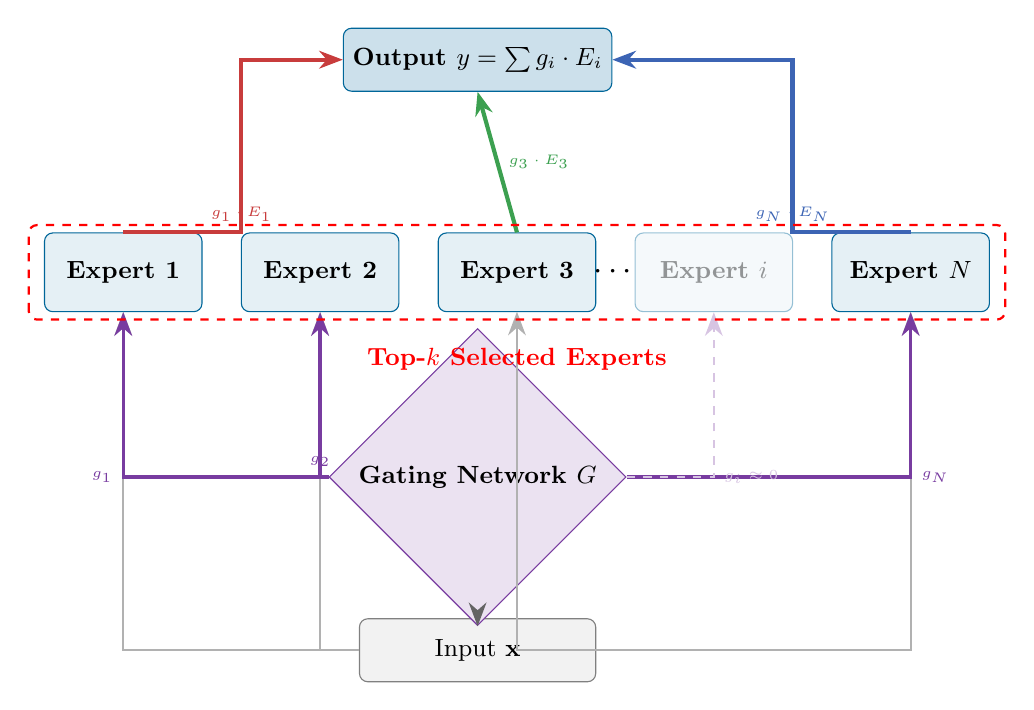
\begin{tikzpicture}[
    expert/.style={rectangle, draw=natureblue, fill=natureblue!10, minimum width=2cm, minimum height=1cm, rounded corners=3pt, font=\small\bfseries},
    gate/.style={diamond, draw=gatepurple, fill=gatepurple!15, minimum width=2.5cm, minimum height=1.5cm, font=\small\bfseries},
    input/.style={rectangle, draw=gray, fill=gray!10, minimum width=3cm, minimum height=0.8cm, rounded corners=3pt, font=\small},
    output/.style={rectangle, draw=natureblue, fill=natureblue!20, minimum width=3cm, minimum height=0.8cm, rounded corners=3pt, font=\small\bfseries},
    arrow/.style={-{Stealth[length=3mm]}, thick, color=naturegray}
]

% Input
\node[input] (input) at (0,0) {Input $\mathbf{x}$};

% Gating Network
\node[gate] (gate) at (0,2.2) {Gating Network $G$};

% Experts
\node[expert] (e1) at (-4.5,4.8) {Expert 1};
\node[expert] (e2) at (-2,4.8) {Expert 2};
\node[expert] (e3) at (0.5,4.8) {Expert 3};
\node[expert, opacity=0.4] (e4) at (3,4.8) {Expert $i$};
\node[expert] (en) at (5.5,4.8) {Expert $N$};

% Dots
\node at (1.75,4.8) {\large$\cdots$};

% Output
\node[output] (output) at (0,7.5) {Output $y = \sum g_i \cdot E_i$};

% Arrows: input to gate
\draw[arrow] (input) -- (gate);

% Arrows: input to experts (data flow)
\draw[arrow, color=naturegray!50] (input.west) -| (-4.5,1.5) -- (-4.5,4.3);
\draw[arrow, color=naturegray!50] (input.west) -| (-2,1.5) -- (-2,4.3);
\draw[arrow, color=naturegray!50] (input.east) -| (0.5,1.5) -- (0.5,4.3);
\draw[arrow, color=naturegray!50] (input.east) -| (5.5,1.5) -- (5.5,4.3);

% Arrows: gate to experts (gating weights) - only top-k
\draw[arrow, color=gatepurple, line width=1.2pt] (gate.west) -| (-4.5,3.5) node[midway, left, font=\tiny, color=gatepurple] {$g_1$} -- (e1.south);
\draw[arrow, color=gatepurple, line width=1.2pt] (gate.west) -| (-2,3.5) node[midway, above, font=\tiny, color=gatepurple] {$g_2$} -- (e2.south);
\draw[arrow, color=gatepurple, line width=1.2pt] (gate.east) -| (5.5,3.5) node[midway, right, font=\tiny, color=gatepurple] {$g_N$} -- (en.south);
\draw[arrow, color=gatepurple!30, dashed] (gate.east) -| (3,3.5) node[midway, right, font=\tiny, color=gatepurple!30] {$g_i \approx 0$} -- (e4.south);

% Arrows: experts to output (only top-k)
\draw[arrow, color=expertsred, line width=1.5pt] (e1.north) -| (-3,6.8) node[midway, above, font=\tiny] {$g_1 \cdot E_1$} |- (output.west);
\draw[arrow, color=expertsgreen, line width=1.5pt] (e3.north) -- (output.south) node[midway, right, font=\tiny] {$g_3 \cdot E_3$};
\draw[arrow, color=expertsblue, line width=1.5pt] (en.north) -| (4,6.8) node[midway, above, font=\tiny] {$g_N \cdot E_N$} |- (output.east);

% Bracket annotation for top-k
\draw[red, dashed, thick, rounded corners=3pt] (-5.7,4.2) rectangle (6.7,5.4);
\node[font=\small\bfseries, color=red] at (0.5,3.7) {Top-$k$ Selected Experts};

\end{tikzpicture}
\caption{\textbf{Architecture of a Mixture of Experts (MoE) model.} The gating network $G$ produces sparse weights $g_i$ for each expert $E_i$. Only the top-$k$ experts (solid purple arrows) are activated for each input, while others (dashed, near-zero weights) remain dormant. The output is the weighted sum of activated expert outputs: $y = \sum_{i \in \text{TopK}} g_i \cdot E_i(\mathbf{x})$.}
\label{fig:moe_architecture}
\end{figure}


\begin{figure}[htbp]
\centering
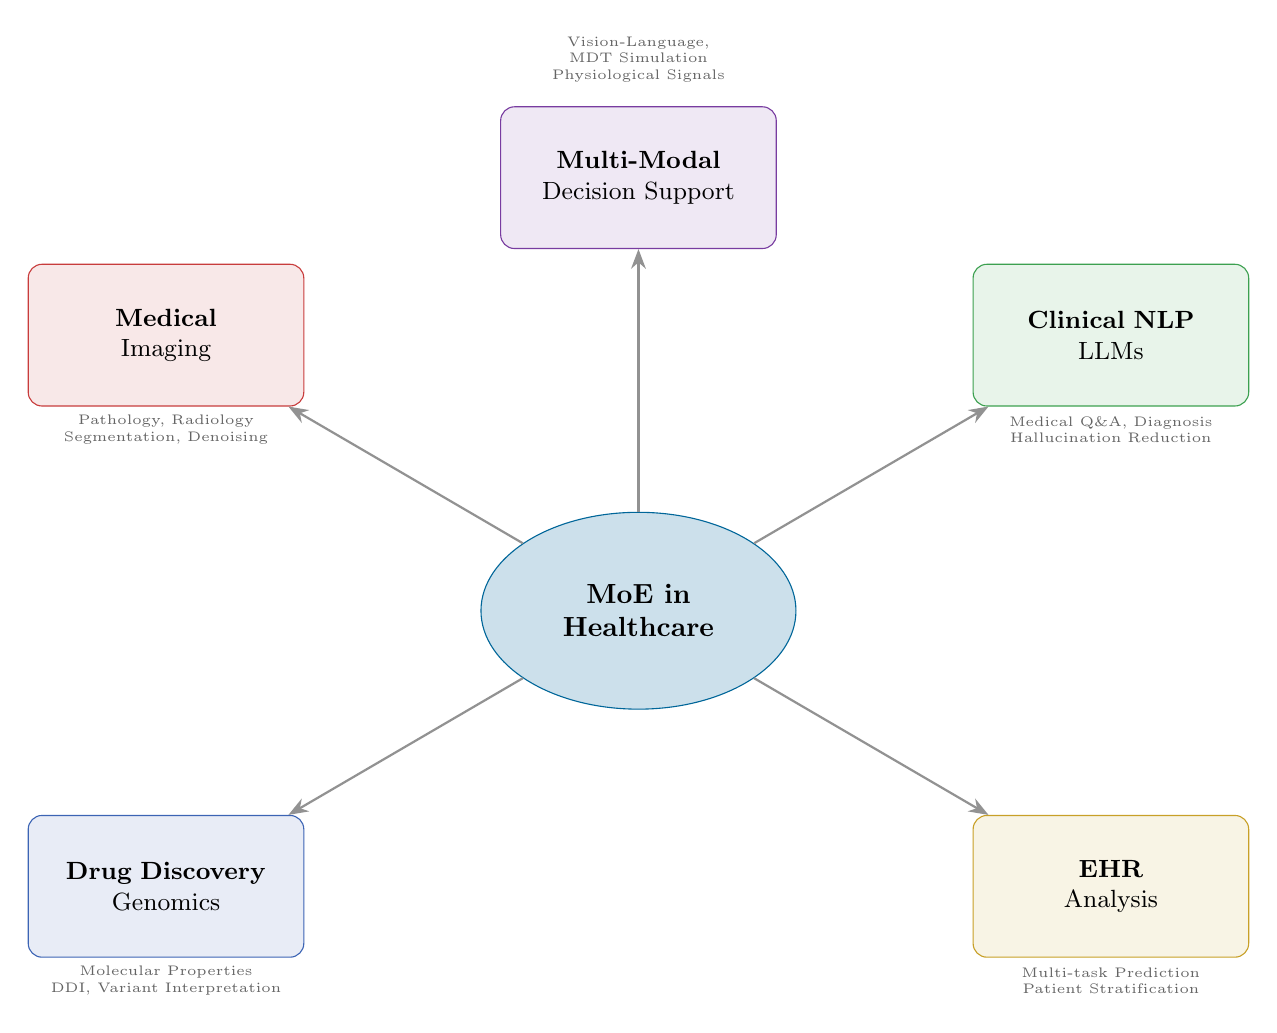
\begin{tikzpicture}[
    domain/.style={rectangle, draw=#1, fill=#1!12, minimum width=3.5cm, minimum height=1.8cm, rounded corners=5pt, text width=3.2cm, align=center, font=\small},
    center/.style={ellipse, draw=natureblue, fill=natureblue!20, minimum width=4cm, minimum height=2.5cm, font=\bfseries, align=center},
    arrow/.style={-{Stealth[length=2.5mm]}, thick, color=naturegray!70}
]

% Center: MoE
\node[center] (moe) at (0,0) {MoE in\\Healthcare};

% Domains
\node[domain=expertsred] (imaging) at (-6,3.5) {\textbf{Medical}\\Imaging};
\node[domain=expertsgreen] (nlp) at (6,3.5) {\textbf{Clinical NLP}\\LLMs};
\node[domain=expertsblue] (drug) at (-6,-3.5) {\textbf{Drug Discovery}\\Genomics};
\node[domain=expertsgold] (ehr) at (6,-3.5) {\textbf{EHR}\\Analysis};
\node[domain=gatepurple] (multi) at (0,5.5) {\textbf{Multi-Modal}\\Decision Support};

% Arrows
\draw[arrow] (moe) -- (imaging);
\draw[arrow] (moe) -- (nlp);
\draw[arrow] (moe) -- (drug);
\draw[arrow] (moe) -- (ehr);
\draw[arrow] (moe) -- (multi);

% Sub-labels
\node[font=\tiny, color=naturegray, text width=3cm, align=center] at (-6,2.3) {Pathology, Radiology\\Segmentation, Denoising};
\node[font=\tiny, color=naturegray, text width=3cm, align=center] at (6,2.3) {Medical Q\&A, Diagnosis\\Hallucination Reduction};
\node[font=\tiny, color=naturegray, text width=3cm, align=center] at (-6,-4.7) {Molecular Properties\\DDI, Variant Interpretation};
\node[font=\tiny, color=naturegray, text width=3cm, align=center] at (6,-4.7) {Multi-task Prediction\\Patient Stratification};
\node[font=\tiny, color=naturegray, text width=3.5cm, align=center] at (0,7) {Vision-Language, MDT Simulation\\Physiological Signals};

\end{tikzpicture}
\caption{\textbf{Overview of MoE applications across healthcare domains.} The Mixture of Experts architecture has been applied to five major areas of healthcare AI: medical imaging (including computational pathology and radiology), clinical NLP and medical LLMs, drug discovery and genomics, electronic health record analysis, and multi-modal clinical decision support.}
\label{fig:healthcare_overview}
\end{figure}


% ---- Tables ----
\clearpage
\section*{Tables}
\addcontentsline{toc}{section}{Tables}


\begin{table}[htbp]
\centering
\caption{\textbf{Summary of MoE applications across healthcare domains.}}
\label{tab:moe_summary}
\small
\begin{tabular}{@{}p{2cm}p{3.5cm}p{4cm}p{3.5cm}@{}}
\toprule
\textbf{Domain} & \textbf{Application} & \textbf{MoE Approach} & \textbf{Key Innovation} \\
\midrule
\multirow{3}{2cm}{Medical Imaging} & Pathology blur robustness & Multi-expert with quality-aware gating & Variable-blur expert training \citep{xie2024moe_pathology} \\
\cmidrule(lr){2-4}
& Multi-site segmentation & Personalized site-specific experts & Adaptive site routing \citep{rahman2025personalized_moe} \\
\cmidrule(lr){2-4}
& Brain tumor segmentation & Modality-specific experts for MRI & Adaptive multi-modal gating \citep{kim2026amoe_bts} \\
\midrule
\multirow{2}{2cm}{Clinical NLP} & Breast cancer support & LoRA experts with knowledge routing & Hallucination mitigation \citep{bechar2025biocancer_moe} \\
\cmidrule(lr){2-4}
& MDT simulation & Discipline-specific expert reasoning & Collaborative consensus \citep{chen2026cor_mole} \\
\midrule
\multirow{2}{2cm}{Drug Discovery} & Epigenetic analysis & Mark-specific MoE Transformer & Multi-epigenomic integration \citep{acharya2025mobius} \\
\cmidrule(lr){2-4}
& Single-cell multi-omics & Sparse MoE for modalities & Cross-modal cell representation \citep{yun2024scmoe} \\
\midrule
\multirow{1}{2cm}{Multi-Modal} & Multi-pathology diagnosis & Sparse MoE vision-language & Pathology-specific experts \citep{khan2025medvlmoe} \\
\bottomrule
\end{tabular}
\end{table}


\begin{table}[htbp]
\centering
\caption{\textbf{Comparison of major MoE architectural variants and their healthcare relevance.}}
\label{tab:moe_variants}
\small
\begin{tabular}{@{}p{2.8cm}p{1.5cm}p{2cm}p{2.5cm}p{3.5cm}@{}}
\toprule
\textbf{Architecture} & \textbf{Experts} & \textbf{Routing} & \textbf{Key Feature} & \textbf{Healthcare Relevance} \\
\midrule
Original MoE \citep{jacobs1991adaptive} & Few & Soft gating & Modular decomposition & Patient stratification \\
\midrule
Sparse MoE \citep{shazeer2017outrageously} & Many & Top-$k$ & Conditional computation & Large-scale medical LLMs \\
\midrule
Switch Transformer \citep{fedus2022switch} & Many & Top-1 & Simplified routing & Efficient clinical inference \\
\midrule
Mixtral \citep{jiang2024mixtral} & 8 & Top-2 & Open-weight MoE & Medical NLP fine-tuning \\
\midrule
DeepSeek-MoE \citep{dai2024deepseekmoe} & Fine-grained & Top-$k$ & Shared + routed experts & Multi-task clinical prediction \\
\midrule
MoELoRA \citep{rai2024moe_lora} & Few & Learned gating & Parameter-efficient & Low-resource medical adaptation \\
\bottomrule
\end{tabular}
\end{table}


% ---- References ----
\clearpage
\section*{References}
\addcontentsline{toc}{section}{References}
\bibliographystyle{plainnat}
\bibliography{refs}

\end{document}
